\section*{4/20}
  \subsection*{Markov Chain}
    Determined by
    \begin{itemize}
      \item \underline{state space}: a countable set, often represented
        by positive numbers.
      \item \underline{transition probabilities}
        $$
          P_{ij} = P(X_{n+1} = j | X_n = i)
        $$
        which satisfy $P_{ij} \ge 0$, $\sum_j P_{ij}, \forall i$
      \item \underline{initial state}
    \end{itemize}
    Graphically, one often represents a Markov Chain like this:\\
    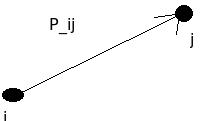
\includegraphics{4_20.jpeg}\\
    $$
      P_{ij}^n = P(X_n = j | X_0 = i) (= P(X_{n+m} = j | X_m = i))
    $$
    $$
      P_{ij}^1 = P{ij}
    $$
    This is called the \emph{n-step probabilities}.\\
    \begin{eqnarray*}
      P_{ij}^{n+m} & = & P(X_{n+m} = j | X_0 = i)\\
        & = & \sum_k P(X_{n+m} = j, X_n = k | X_0 = i) \text{ ($X_0 =i$ isn't really a condition. It's just the starting state)}\\
        & = & P(X_{n+m} = j | X_n= k)P(X_n = k | X_0 = i) \\
        & = & P(X_{m} = j | X_0= k)P(X_n = k | X_0 = i) \text{ (doesn't matter how you got there.)}\\
        & = & \sum_k P_{kj}^m P_{ik}^n \\
    \end{eqnarray*}
    Let $P^{(n)}$ be the matrix, $P_{ij}^n$
    \begin{eqnarray*}
      P^{(m+n)}  & = & P^{(n)}P^{(m)} \\
      P^{(n)} & = & P^{(1)}P^{(1)} \ldots P^{(1)}\\
        & = & P^n
    \end{eqnarray*}
    Conclusion: Computing $n$-step transition probability is the same as
    computing powers of $P$.\\

    \noindent \underline{Example}: Two state Markov Chain defined by
    $$
      P = \left[\begin{array}{c c} \alpha & 1 - \alpha\\ \beta & 1 - \beta
        \end{array}\right]
    $$
    Then,
    $$
      P^2 = \left[\begin{array}{c c} \alpha^2 + (1 - \alpha)\beta 
        & \alpha(1 - \alpha) + (1 -\alpha) (1 - \beta)\\ 
        \alpha\beta + (1 - \beta)\beta 
        & \beta(1 - \alpha) + (1 - \beta)^2
        \end{array}\right]
    $$
    Assume now, that initial distribution is given by
    $$
      \alpha_i = P(X_0 = i), \forall i, (\sum_i \alpha_i = 1, \alpha_i \ge 0)
    $$
    \begin{eqnarray*}
      P(X_n = j) & = & \sum_i P(X_n = j | X_0 = i)P(X_0 = i)\\
        & = & \sum_i \alpha_i P_{ij}^n\\
    \end{eqnarray*}
    The row of probabilities is given by
    $$
      P(X_n = i) = [\alpha_0, \alpha_1, \ldots ]P^n
    $$

    \noindent\underline{Example}: Random walk on the graph below:\\
    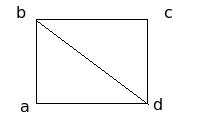
\includegraphics{4_20_2.jpeg}\\
    Choose starting point at random. What is the probability that a random
    walk is at $a$ after 2 steps. At each vertex, you are equally likely to
    choose any of the edges it is connected to.\\
    $$
      P = \left[\begin{array}{c c c c}
        0 &  \frac{1}{2} & 0 & \frac{1}{2}\\
        \frac{1}{3} & 0 & \frac{1}{3} & \frac{1}{3}\\
        0 & \frac{1}{2} & 0 & \frac{1}{2}\\
        \frac{1}{3} & \frac{1}{3} & \frac{1}{3} & 0
        \end{array}\right]
    $$
    $$
      \left[\begin{array}{c c c c} \frac{1}{4} & \frac{1}{4} & \frac{1}{4}
        & \frac{1}{4}\end{array}\right] P^2 = \left[\begin{array}{c c c c} P(X_2 = 1) & P(X_2 = 2) & P(X_2 = 3) & P(X_2 = 4)\end{array}\right]
    $$
  \subsection*{Classification of states}
    \begin{itemize}
      \item We say that a state $j$ is \underline{accessible from state $i$}
        if $P_{ij}^n > 0$ for some $n > 0$. (there is a possibility of 
        reaching $j$ from $i$ in any number of steps).
      \item If $i$ is accessible from $j$, and $j$ is accessible from $i$,
        then we say that $i$ and $j$ are \underline{coummunicate}, $i 
        \leftrightarrow j$
      \item "$\leftrightarrow$" is an \underline{equivalence relation}.
        \begin{itemize}
          \item $i \leftrightarrow i$
          \item $i \leftrightarrow j \Rightarrow j \leftrightarrow i$
          \item $i \leftrightarrow j$ and $j \leftrightarrow k \Rightarrow i \leftrightarrow k$
        \end{itemize}
    \end{itemize}
    \underline{Example}:\\ 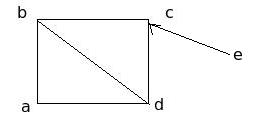
\includegraphics{4_20_3.jpeg}\\
    Any state, $a, b, c, d$ is accessible from $e$, but $e$ is not accessible
    from $a, b, c, d$.\\
    $e$ is accessible from $e$ by definition.\\
